% Options for packages loaded elsewhere
% Options for packages loaded elsewhere
\PassOptionsToPackage{unicode}{hyperref}
\PassOptionsToPackage{hyphens}{url}
\PassOptionsToPackage{dvipsnames,svgnames,x11names}{xcolor}
%
\documentclass[
  number,
  review,
  3p]{elsarticle}
\usepackage{xcolor}
\usepackage{amsmath,amssymb}
\setcounter{secnumdepth}{5}
\usepackage{iftex}
\ifPDFTeX
  \usepackage[T1]{fontenc}
  \usepackage[utf8]{inputenc}
  \usepackage{textcomp} % provide euro and other symbols
\else % if luatex or xetex
  \usepackage{unicode-math} % this also loads fontspec
  \defaultfontfeatures{Scale=MatchLowercase}
  \defaultfontfeatures[\rmfamily]{Ligatures=TeX,Scale=1}
\fi
\usepackage{lmodern}
\ifPDFTeX\else
  % xetex/luatex font selection
\fi
% Use upquote if available, for straight quotes in verbatim environments
\IfFileExists{upquote.sty}{\usepackage{upquote}}{}
\IfFileExists{microtype.sty}{% use microtype if available
  \usepackage[]{microtype}
  \UseMicrotypeSet[protrusion]{basicmath} % disable protrusion for tt fonts
}{}
\makeatletter
\@ifundefined{KOMAClassName}{% if non-KOMA class
  \IfFileExists{parskip.sty}{%
    \usepackage{parskip}
  }{% else
    \setlength{\parindent}{0pt}
    \setlength{\parskip}{6pt plus 2pt minus 1pt}}
}{% if KOMA class
  \KOMAoptions{parskip=half}}
\makeatother
% Make \paragraph and \subparagraph free-standing
\makeatletter
\ifx\paragraph\undefined\else
  \let\oldparagraph\paragraph
  \renewcommand{\paragraph}{
    \@ifstar
      \xxxParagraphStar
      \xxxParagraphNoStar
  }
  \newcommand{\xxxParagraphStar}[1]{\oldparagraph*{#1}\mbox{}}
  \newcommand{\xxxParagraphNoStar}[1]{\oldparagraph{#1}\mbox{}}
\fi
\ifx\subparagraph\undefined\else
  \let\oldsubparagraph\subparagraph
  \renewcommand{\subparagraph}{
    \@ifstar
      \xxxSubParagraphStar
      \xxxSubParagraphNoStar
  }
  \newcommand{\xxxSubParagraphStar}[1]{\oldsubparagraph*{#1}\mbox{}}
  \newcommand{\xxxSubParagraphNoStar}[1]{\oldsubparagraph{#1}\mbox{}}
\fi
\makeatother


\usepackage{longtable,booktabs,array}
\usepackage{calc} % for calculating minipage widths
% Correct order of tables after \paragraph or \subparagraph
\usepackage{etoolbox}
\makeatletter
\patchcmd\longtable{\par}{\if@noskipsec\mbox{}\fi\par}{}{}
\makeatother
% Allow footnotes in longtable head/foot
\IfFileExists{footnotehyper.sty}{\usepackage{footnotehyper}}{\usepackage{footnote}}
\makesavenoteenv{longtable}
\usepackage{graphicx}
\makeatletter
\newsavebox\pandoc@box
\newcommand*\pandocbounded[1]{% scales image to fit in text height/width
  \sbox\pandoc@box{#1}%
  \Gscale@div\@tempa{\textheight}{\dimexpr\ht\pandoc@box+\dp\pandoc@box\relax}%
  \Gscale@div\@tempb{\linewidth}{\wd\pandoc@box}%
  \ifdim\@tempb\p@<\@tempa\p@\let\@tempa\@tempb\fi% select the smaller of both
  \ifdim\@tempa\p@<\p@\scalebox{\@tempa}{\usebox\pandoc@box}%
  \else\usebox{\pandoc@box}%
  \fi%
}
% Set default figure placement to htbp
\def\fps@figure{htbp}
\makeatother





\setlength{\emergencystretch}{3em} % prevent overfull lines

\providecommand{\tightlist}{%
  \setlength{\itemsep}{0pt}\setlength{\parskip}{0pt}}



 
\usepackage[]{natbib}
\bibliographystyle{elsarticle-num}


\usepackage{booktabs}
\usepackage{caption}
\usepackage{longtable}
\usepackage{colortbl}
\usepackage{array}
\usepackage{anyfontsize}
\usepackage{multirow}
\makeatletter
\@ifpackageloaded{tcolorbox}{}{\usepackage[skins,breakable]{tcolorbox}}
\@ifpackageloaded{fontawesome5}{}{\usepackage{fontawesome5}}
\definecolor{quarto-callout-color}{HTML}{909090}
\definecolor{quarto-callout-note-color}{HTML}{0758E5}
\definecolor{quarto-callout-important-color}{HTML}{CC1914}
\definecolor{quarto-callout-warning-color}{HTML}{EB9113}
\definecolor{quarto-callout-tip-color}{HTML}{00A047}
\definecolor{quarto-callout-caution-color}{HTML}{FC5300}
\definecolor{quarto-callout-color-frame}{HTML}{acacac}
\definecolor{quarto-callout-note-color-frame}{HTML}{4582ec}
\definecolor{quarto-callout-important-color-frame}{HTML}{d9534f}
\definecolor{quarto-callout-warning-color-frame}{HTML}{f0ad4e}
\definecolor{quarto-callout-tip-color-frame}{HTML}{02b875}
\definecolor{quarto-callout-caution-color-frame}{HTML}{fd7e14}
\makeatother
\makeatletter
\@ifpackageloaded{caption}{}{\usepackage{caption}}
\AtBeginDocument{%
\ifdefined\contentsname
  \renewcommand*\contentsname{Table of contents}
\else
  \newcommand\contentsname{Table of contents}
\fi
\ifdefined\listfigurename
  \renewcommand*\listfigurename{List of Figures}
\else
  \newcommand\listfigurename{List of Figures}
\fi
\ifdefined\listtablename
  \renewcommand*\listtablename{List of Tables}
\else
  \newcommand\listtablename{List of Tables}
\fi
\ifdefined\figurename
  \renewcommand*\figurename{Figure}
\else
  \newcommand\figurename{Figure}
\fi
\ifdefined\tablename
  \renewcommand*\tablename{Table}
\else
  \newcommand\tablename{Table}
\fi
}
\@ifpackageloaded{float}{}{\usepackage{float}}
\floatstyle{ruled}
\@ifundefined{c@chapter}{\newfloat{codelisting}{h}{lop}}{\newfloat{codelisting}{h}{lop}[chapter]}
\floatname{codelisting}{Listing}
\newcommand*\listoflistings{\listof{codelisting}{List of Listings}}
\makeatother
\makeatletter
\makeatother
\makeatletter
\@ifpackageloaded{caption}{}{\usepackage{caption}}
\@ifpackageloaded{subcaption}{}{\usepackage{subcaption}}
\makeatother
\journal{Journal Name}
\usepackage{bookmark}
\IfFileExists{xurl.sty}{\usepackage{xurl}}{} % add URL line breaks if available
\urlstyle{same}
\hypersetup{
  pdftitle={Responsive Robotics to Increase Trust in Autonomous Human--Robot Interaction},
  pdfauthor={M.C. Lau; Shauna Heron},
  pdfkeywords={human-robot collaboration, HRI, HRC, socially assistive
robotics, cobots, autonomous robot systems, spoken language
interaction, trust in automation, trust in human-robot
interaction, affect-adaptive systems},
  colorlinks=true,
  linkcolor={blue},
  filecolor={Maroon},
  citecolor={Blue},
  urlcolor={Blue},
  pdfcreator={LaTeX via pandoc}}


\setlength{\parindent}{6pt}
\begin{document}

\begin{frontmatter}
\title{Responsive Robotics to Increase Trust in Autonomous Human--Robot
Interaction \\\large{An In-Person Pilot Study} }
\author[1]{M.C. Lau%
\corref{cor1}%
\fnref{fn1}}
 \ead{mclau@laurentian.ca} 
\author[1]{Shauna Heron%
%
\fnref{fn2}}
 \ead{sheron@laurentian.ca} 

\affiliation[1]{organization={Laurentian University, Bharti School of
Engineering},,postcodesep={}}
\affiliation[2]{organization={Laurentian University, School of Social
Sciences},,postcodesep={}}

\cortext[cor1]{Corresponding author}
\fntext[fn1]{This is the first author footnote.}
\fntext[fn2]{Another author footnote, this is a very long footnote and
it should be a really long footnote. But this footnote is not yet
sufficiently long enough to make two lines of footnote text.}
        
\begin{abstract}
This study implements a multi-stage collaborative task system where
participants collaborate with the Misty-II social robot to solve a
who-dunnit type task. The system utilizes an autonomous,
mixed-initiative dialogue architecture with affect-responsive
capabilities.
\end{abstract}





\begin{keyword}
    human-robot collaboration \sep HRI \sep HRC \sep socially assistive
robotics \sep cobots \sep autonomous robot systems \sep spoken language
interaction \sep trust in automation \sep trust in human-robot
interaction \sep 
    affect-adaptive systems
\end{keyword}
\end{frontmatter}
    

\section{Introduction}\label{introduction}

As automation expands across safety-critical domains such as
manufacturing, mining, and healthcare, robotic systems are increasingly
expected to operate alongside humans rather than in isolation
\citep{fu2021, ciuffreda2025, diab2025, spitale2023}. In these
collaborative settings, successful deployment depends not only on
technical performance and safety guarantees, but on whether human users
are willing to rely on, communicate with, and coordinate their actions
around systems driven by artificial intelligence (AI)
\citep{campagna2025, emaminejad2022}. Trust has therefore emerged as a
central determinant of adoption and effective use in human--robot
collaboration (HRC) \citep{wischnewski2023, campagna2025}. Insufficient
trust can lead to disuse or rejection of automation, while excessive
trust risks overreliance---particularly in environments characterized by
uncertainty or incomplete information \citep{devisser2020}.

A substantial body of human--robot interaction (HRI) research has
examined how robot behaviour shapes user trust, perceived reliability,
and cooperation across industrial and social contexts
\citep{shayganfar2019, fartook2025}. Trust is commonly conceptualized as
a multidimensional construct encompassing cognitive evaluations of
competence and reliability, affective responses to the interaction
partner, and behavioural willingness to rely on the system under
conditions of risk or uncertainty
\citep{muir1994, hancock2011, devisser2020}. Despite this
multidimensional framing, empirical studies have predominantly
operationalized trust using post-interaction self-report questionnaires,
often collected following short, highly controlled interactions.

Importantly, much of the existing HRI trust literature relies on
scripted behaviours, simulated environments, or Wizard-of-Oz paradigms
in which a human operator covertly manages the robot's behaviour. While
these approaches are valuable for isolating specific design factors,
they obscure the interaction breakdowns and system imperfections that
characterize real-world autonomous robots \citep{campagna2025}. In
deployed systems, limitations such as speech recognition errors, delayed
responses, misinterpretations of user intent, and incomplete affect
sensing are not peripheral issues but defining features of interaction.
These failures are likely to play a decisive role in shaping trust and
collaboration, yet remain underrepresented in empirical evaluations.

One proposed mechanism for supporting trust in HRI is responsiveness:
the extent to which a robot adapts its behaviour based on user state and
interaction context \citep{shayganfar2019, fartook2025}. Responsive
robots may adjust dialogue, timing, or support strategies in response to
inferred cues such as confusion, frustration, or disengagement, and
prior work suggests that such adaptive behaviour can enhance perceived
social intelligence and trustworthiness in dialogue-driven tasks
\citep{birnbaum2016}. However, most evidence for these effects comes
from simulated or semi-autonomous systems, leaving open questions about
how responsiveness operates when implemented in fully autonomous,
in-person interactions subject to real-time constraints and failure
\citep{campagna2025}.

From an engineering perspective, responsiveness represents an
interaction policy rather than a superficial social cue
\citep{shayganfar2019}. Proactive assistance based on interaction
context differs fundamentally from reactive, request-based behaviour,
particularly in fully autonomous systems---for example, offering
clarification or encouragement when confusion or hesitation is inferred,
rather than waiting for an explicit request for help
\citep{birnbaum2016}. Implementing such policies requires robots to
manage spoken-language dialogue, track interaction state over time, and
coordinate verbal and nonverbal responses in real time, all while
operating under noise, latency, and sensing uncertainty
\citep{campagna2025}.

The present work addresses these gaps through a pilot study examining
trust and collaboration during in-person interaction with a fully
autonomous social robot. Participants collaborated with one of two
versions of the same robot platform during a dialogue-driven puzzle task
requiring shared problem solving. In both conditions, all interaction
management---including speech recognition, dialogue state tracking, task
progression, and response generation---was handled and logged
autonomously by the robot without human intervention. In the responsive
condition, the robot employed a proactive interaction policy, adapting
its assistance based on conversational cues and inferred user affect. In
the neutral condition, the robot followed a reactive policy, providing
general guidance but assistance only when explicitly requested.

This pilot study had three primary objectives: (1) to design and
evaluate the feasibility of an autonomous spoken-language interaction
system with affect-responsive behaviour on a mobile robot platform; (2)
to assess whether interaction policy influences post-interaction trust
and collaborative experience under realistic autonomous conditions; and
(3) to explore how behavioural and interaction-level indicators align
with subjective trust evaluations. Rather than optimizing for flawless
interaction, the system was intentionally designed to reflect the
capabilities and limitations of contemporary social robots, allowing
interaction breakdowns to surface naturally.

By combining post-interaction trust measures with task-level and
behavioural observations, this study aims to contribute empirical
evidence on how trust in human--robot collaboration emerges and is
enacted during fully autonomous interaction. The findings are intended
to inform the design of a larger subsequent study by evaluating
feasibility and identifying technical, interactional, and methodological
challenges that must be addressed when evaluating affect-responsive
robots in real-world contexts.

\section{Methods}\label{methods}

\subsection{Experimental Design and
Conditions}\label{experimental-design-and-conditions}

This study employed a between-subjects experimental design to examine
how robot interaction policy influences trust and collaboration during
fully autonomous, in-person human--robot interaction. The sole
experimental factor was the robot's interaction policy, with
participants randomly assigned to interact with either a responsive or
neutral version of the same robot system.

Throughout this paper, references to \emph{the robot} denote the fully
autonomous interactive system comprising the Misty-II hardware platform
and its onboard software stack, with all interaction decisions generated
without human intervention, including spoken-language processing,
dialogue management, and the interaction policy governing verbal and
nonverbal behaviour. Additional details of the system architecture are
provided in Appendix A.

Participants interacted with a Misty-II social robot in a shared
physical workspace that included a participant-facing computer interface
\citep{mistyrobotics}. The interface was used to display task materials,
collect participant inputs, and manage task progression (see
Figure~\ref{fig-task1}). Importantly, the interface did not function as
a control mechanism for the robot. Instead, the robot autonomously
monitored task state and participant inputs via the interface and
managed dialogue and behaviour accordingly, without real-time human
intervention.

\subsubsection*{Interaction Policies}\label{interaction-policies}
\addcontentsline{toc}{subsubsection}{Interaction Policies}

\begin{itemize}
\item
  \textbf{Responsive condition (experimental):}\\
  The robot employed a proactive, affect-adaptive interaction policy.
  Robot responses were modulated based on inferred participant affect,
  dialogue context, and task demands, resulting in unsolicited
  encouragement, clarification, and engagement-oriented behaviours when
  appropriate.
\item
  \textbf{Control condition (baseline):}\\
  The robot employed a neutral, reactive interaction policy. General
  information and guidance were were provided but additional help only
  when explicitly requested by the participant and without affect-based
  adaptation or proactive support beyond a check-in when participant was
  silent for more than 1 minute.
\end{itemize}

Both conditions used identical hardware, software infrastructure,
sensing capabilities, and task logic. The only difference between
conditions was the robot's interaction policy.

\subsection{Collaborative Task Design}\label{collaborative-task-design}

Participants completed an immersive, narrative-driven puzzle game
consisting of five sequential stages and two timed reasoning tasks. The
game context positioned participants as investigators searching for a
missing robot colleague, with the robot serving as a diegetic guide and
collaborative partner. The overall interaction lasted approximately 25
minutes.

\begin{figure}

\centering{

\includegraphics[width=5.02083in,height=\textheight,keepaspectratio]{images/misty-pullback.jpg}

}

\caption{\label{fig-setup}Experimental setup showing the autonomous
robot and participant-facing task interface used during in-person
sessions. Participants entered task responses and navigated between task
stages using the interface, while the robot autonomously tracked task
state and adapted its interaction based on participant input.}

\end{figure}%

The task structure was designed to elicit collaboration under two
distinct dependency conditions: (1) enforced collaboration, where the
robot was required to complete the task, and (2) optional collaboration,
where participants could choose whether to engage the robot.

\textbf{Stage Overview}

\begin{enumerate}
\def\labelenumi{\arabic{enumi}.}
\tightlist
\item
  \textbf{Greeting:} The robot introduced itself and engaged in brief
  rapport-building dialogue.\\
\item
  \textbf{Mission Brief:} The robot explained the narrative context and
  overall objectives.\\
\item
  \textbf{Task 1:} Robot-dependent collaborative reasoning task.\\
\item
  \textbf{Task 2:} Open-ended problem solving with optional robot
  support.\\
\item
  \textbf{Wrap-up:} The robot provided closing feedback and concluded
  the interaction.
\end{enumerate}

Participants advanced between stages using the interface, either at the
robot's prompting or at their own discretion. All spoken dialogue and
interaction events were logged automatically.

\subsubsection{Task 1: Robot-Dependent Collaborative
Reasoning}\label{task-1-robot-dependent-collaborative-reasoning}

In Task 1, participants were asked to identify a perpetrator from a 6 ×
4 grid of 24 `suspects' by asking the robot a series of yes/no questions
about the suspect's features (e.g., ``was the suspect wearing a hat?'').
The grid was displayed on the interface, while questions were posed
verbally.

\begin{figure}

\includegraphics[width=5.02083in,height=\textheight,keepaspectratio]{images/task1-whodunnit2.png}

\caption{\label{fig-task1}\emph{Task 1 interface including the 6 × 4
grid of 24 candidates. Participants could track those eliminated by
clicking on subjects which would grey them out. A box was provided to
input their final answer and a button included to move to the Task 2
interface.}}

\end{figure}%

The robot possessed ground-truth information necessary to answer each
question correctly. Successful task completion was therefore dependent
on interaction with the robot, creating a forced collaborative dynamic.
Participants were required to coordinate questioning strategies with the
robot to narrow down the suspect within a five-minute time limit. The
structured nature of the task ensured consistent interaction demands
across participants and conditions.

\subsubsection{Task 2: Open-Ended Collaborative Problem
Solving}\label{task-2-open-ended-collaborative-problem-solving}

Task 2 involved a more open-ended reasoning challenge. Participants were
presented with multiple technical logs through a simulated terminal
interface that could be used to infer the location of the missing robot.

\begin{figure}

\centering{

\includegraphics[width=5.02083in,height=\textheight,keepaspectratio]{images/task2-cryptic-puzzle.png}

}

\caption{\label{fig-task2}The task 2 interface presented multiple
technical logs through a simulated terminal interface that could be used
to determine the location of the missing robot.}

\end{figure}%

Unlike Task 1, the robot did not have access to ground-truth information
or the contents of the logs. The robot's assistance was limited to
general reasoning support derived from its language model, such as
explaining how to interpret log formats, suggesting problem-solving
strategies, or prompting participants to reflect on inconsistencies.

Participants could complete this task independently or solicit
assistance from the robot at their discretion \citep{lin2022}. This
design allowed collaboration to emerge voluntarily rather than being
enforced by task structure, positioning the robot as a collaborative
partner rather than an authoritative source.

\subsection{Study Protocol}\label{study-protocol}

Participants signed up for the study and completed a pre-session
questionnaire before their in-person session via Qualtrics. The
pre-session questionnaire colleced basic demographics information and
assessed baseline characteristics, including the Negative Attitudes
Toward Robots Scale (NARS) and the short form of the Need for Cognition
scale (NFC-s). These measures were used to capture individual
differences that may moderate responses to robot interaction.

In-person sessions were conducted in a quiet, private room at Laurentian
University between November and December 2025. Prior to each session,
the robot's interaction policy was configured to the assigned
experimental condition.

Upon arrival, participants were greeted by the researcher, provided with
a brief overview of the session, and given instructions for effective
communication with the robot, including waiting for a visual indicator
before speaking. Once participants indicated readiness, the researcher
exited the room, leaving the participant and robot to complete the
interaction without human presence or observation. Participants
initiated the interaction by clicking a start button on the interface
and were informed that they could terminate the session at any time
without penalty.

Following task completion, participants completed a 21-item
post-interaction questionnaire assessing trust. Participants then
engaged in a brief debrief with the researcher and were awarded a \$15
gift card. Total session duration averaged approximately 30 minutes.

\subsection{Measures}\label{measures}

A combination of self-report and objective measures was used to assess
trust, engagement, and task performance.

\subsubsection{Self-Report Measures}\label{self-report-measures}

Trust was assessed using two established self-report instruments
commonly used in human--robot interaction research: the Trust Perception
Scale--HRI (TPS-HRI) and the Trust in Industrial Human--Robot
Collaboration scale (TI-HRC) \citep{bartneck2009, charalambous2016}.
Both measures were adapted to reflect the specific task context and
interaction modality of the present study. 9 items were retained from
the TI-HRC and 12 items from the TPS-HRI. Item wording was modified to
reference the robot's behaviour during a dialogue-driven collaborative
task, and response formats were adjusted to ensure interpretability for
participants without prior robotics experience.

Together, these instruments capture complementary dimensions of trust,
including perceived reliability, task competence, and affective comfort.
However, they differ in their conceptual emphasis: the TPS-HRI primarily
operationalizes trust as a reflective judgement of system performance
(i.e., ``What percent of the time was the robot reliable''), whereas the
TI-HRC scale emphasizes trust as an experienced, embodied response
arising during interaction (i.e., ``The way the robot moved made me feel
uneasy''). Despite this complementarity, both measures rely on
retrospective self-report and may be insensitive to moment-to-moment
trust dynamics as collaboration unfolds. For this reason, questionnaire
data were interpreted alongside behavioural and interaction-level
measures.

Participants completed a pre-session questionnaire assessing baseline
characteristics, including the Negative Attitudes Toward Robots Scale
(NARS) and the short form of the Need for Cognition scale (NFC-s). These
measures were used to capture individual differences that may moderate
responses to robot interaction.

\subsubsection{Objective and behavioural
Measures}\label{objective-and-behavioural-measures}

Objective task metrics included task completion, task accuracy, time to
completion, and the number of assistance requests made to the robot.
behavioural engagement metrics were derived from interaction logs and
manually coded dialogue transcripts, including number of dialogue turns,
frequency of communication breakdowns, response timing, and
task-relevant robot contributions.

\subsection{Participants}\label{participants}

A total of 29 participants were recruited from the Laurentian University
community via word of mouth and the SONA recruitment system. Eligibility
criteria included being 18 years or older, fluent in spoken and written
English, and having normal or corrected-to-normal hearing and vision.
Participants received a \$15 gift card as compensation for their time.
All procedures were approved by the Laurentian University Research
Ethics Board (REB \#6021966).

\begin{table}

\caption{\label{tbl-pre}}

\centering{

\fontsize{10.0pt}{12.0pt}\selectfont
\begin{tabular*}{\linewidth}{@{\extracolsep{\fill}}lcccc}
\toprule
\textbf{Characteristic} & \textbf{N} & \textbf{CONTROL}  N = 13\textsuperscript{\textit{1}} & \textbf{RESPONSIVE}  N = 16\textsuperscript{\textit{1}} & \textbf{p-value}\textsuperscript{\textit{2}} \\ 
\midrule\addlinespace[2.5pt]
{\bfseries Gender} & 27 &  &  & 0.84 \\ 
    Woman &  & 6 / 13 (46\%) & 7 / 14 (50\%) &  \\ 
    Man &  & 7 / 13 (54\%) & 7 / 14 (50\%) &  \\ 
{\bfseries Age Group} & 27 &  &  & 0.35 \\ 
    18-24 &  & 5 / 13 (38\%) & 7 / 14 (50\%) &  \\ 
    25-34 &  & 4 / 13 (31\%) & 2 / 14 (14\%) &  \\ 
    34-44 &  & 1 / 13 (7.7\%) & 4 / 14 (29\%) &  \\ 
    45+ &  & 3 / 13 (23\%) & 1 / 14 (7.1\%) &  \\ 
{\bfseries Program} & 25 &  &  & >0.99 \\ 
    Psychology &  & 1 / 13 (7.7\%) & 1 / 12 (8.3\%) &  \\ 
    Engineering &  & 2 / 13 (15\%) & 1 / 12 (8.3\%) &  \\ 
    Computer Science &  & 7 / 13 (54\%) & 6 / 12 (50\%) &  \\ 
    Earth Sciences &  & 0 / 13 (0\%) & 1 / 12 (8.3\%) &  \\ 
    Other &  & 3 / 13 (23\%) & 3 / 12 (25\%) &  \\ 
{\bfseries Experience w/Robots} & 29 & 7 / 13 (54\%) & 4 / 16 (25\%) & 0.14 \\ 
{\bfseries Native English Speaker} & 29 &  &  & 0.53 \\ 
    Native English &  & 5 / 13 (38\%) & 8 / 16 (50\%) &  \\ 
    Non-Native English &  & 8 / 13 (62\%) & 8 / 16 (50\%) &  \\ 
{\bfseries NARS Overall} & 29 & 38 (8) & 38 (7) & 0.79 \\ 
{\bfseries Need for Cognition} & 29 & 3.62 (0.78) & 3.74 (0.74) & 0.55 \\ 
{\bfseries Dialogue Viability} & 29 &  &  & 0.63 \\ 
    exclude &  & 3 / 13 (23\%) & 2 / 16 (13\%) &  \\ 
    include &  & 10 / 13 (77\%) & 14 / 16 (88\%) &  \\ 
\bottomrule
\end{tabular*}
\begin{minipage}{\linewidth}
\textsuperscript{\textit{1}}n / N (\%); Mean (SD)\\
\textsuperscript{\textit{2}}Pearson's Chi-squared test; Fisher's exact test; Wilcoxon rank sum test\\
\end{minipage}

}

\end{table}%

\subsubsection{Communication Viability}\label{communication-viability}

Although English fluency was an eligibility requirement, in-person
observation during data collection indicated meaningful variability in
participants' functional spoken-language proficiency. The researcher
therefore recorded observed English proficiency for each session in
anticipation of potential speech-based system limitations. Subsequent
post-hoc review of interaction transcripts and system logs revealed that
a subset of sessions exhibited severe and sustained communication
failure. In these cases, automatic speech recognition (ASR) output was
largely unintelligible or fragmented, preventing the robot from
extracting sufficient linguistic content to maintain dialogue, respond
meaningfully to participant queries, or support task progression.
Interaction frequently stalled, participant input went unanswered or was
misinterpreted, and collaborative problem-solving was not feasible.
These sessions reflected a breakdown of language-mediated interaction,
rendering the experimental manipulation inoperative.

Because the study relied fundamentally on spoken-language collaboration,
sessions exhibiting persistent communication failure were classified as
protocol non-adherence and excluded from task-level analyses (n = 5).
Exclusion decisions were based solely on communication viability and
interaction mechanics, not on task outcomes or trust measures.

\subsubsection{Analytic Strategy}\label{analytic-strategy}

To ensure transparency and assess the impact of communication-based
exclusions, analyses were conducted in three stages. First, an
eligible-sample analysis (excluding non-viable sessions) served as the
primary analysis, reflecting interactions in which the spoken-language
protocol and experimental manipulation operated as intended. Second, a
full-sample analysis including all participants was conducted as a
sensitivity analysis to evaluate robustness to communication failures
and protocol deviations. Third, a mechanism-focused analysis compared
included and excluded sessions on interaction-process metrics (e.g., ASR
failure rates, dialogue turn completion, task abandonment) to
characterize how severe communication breakdown alters interaction
dynamics.

While full-sample analyses are informative as robustness checks, trust
measures obtained from sessions with complete communication breakdown
are not interpreted as valid estimates of human--robot trust under
functional interaction. In these cases, the robot was unable to sustain
dialogue or collaborative behaviour, precluding meaningful evaluation of
reliability, competence, or collaborative intent.

Across analyses, participants in the responsive and control conditions
were comparable with respect to demographic characteristics, prior
experience with robots, and baseline attitudes toward robots, including
Negative Attitudes Toward Robots (NARS) and Need for Cognition scores
(see Table~\ref{tbl-pre}) \citep{cacioppo1982}. These patterns were
consistent across both eligible and full samples, indicating successful
random assignment.

\section{Results}\label{results}

Prior to hypothesis testing, interaction sessions were classified based
on communication viability using a dialogue-level metric derived from
system logs and manual coding. Specifically, the proportion of dialogue
turns affected by speech-recognition failure or fragmented utterances
was computed for each session. Sessions in which more than 60\% of
dialogue turns (half of all turns were dependent on human speech) were
characterized by communication breakdown were classified as non-viable
(n=5). This criterion closely matched sessions independently flagged
during administration and reflects cases in which sustained
spoken-language interaction was not possible. Of the 29 completed
sessions, 5 were classified as non-viable due to severe and persistent
communication failure resulting in unintelligble sentence fragments.

Because the experimental manipulation relied on language-mediated
collaboration, analyses were conducted using three complementary
approaches: (1) a primary eligible-sample analysis excluding non-viable
sessions, (2) a full-sample sensitivity analysis including all sessions,
and (3) a mechanism-focused analysis examining how communication
breakdown altered interaction dynamics.

Unless otherwise noted, inferential results reported below refer to the
eligible sample.

\subsection{Primary Analysis: Eligible
Sample}\label{primary-analysis-eligible-sample}

\subsubsection*{Descriptive Outcomes}\label{descriptive-outcomes}
\addcontentsline{toc}{subsubsection}{Descriptive Outcomes}

Descriptive comparisons of post-interaction trust measures indicated
higher trust ratings in the responsive condition relative to the control
condition across both trust scales (see Table~\ref{tbl-post-eligible}).
Average post-interaction scores on the TI-HRC differed by approximately
26 points (Likert 1-5 converted to 0-100 scale for easier comparison
across scales). While differences in TPS-HRI scores were approximately
15 points higher in the responsive condition compared to the control.
Scores on the Behavioural summaries further indicated differences in
dialogue patterns and robot assistance behaviours consistent with the
intended interaction policies. TO DO: ADD DIALOGUE ANALYSES STATS

Importantly objective task accuracy did not differ between conditions
across any task-level measures. This suggests that observed differences
in trust were not driven by differential task success.

Despite similar task accuracy, interactions in the responsive condition
were expectedly characterized by longer durations (more dialogue),
slower robot response times (more dialogue), and a higher number of
AI-detected engaged responses. These findings suggest that
responsiveness altered the interaction dynamics and affective tone
rather than task outcomes.

\begin{table}

\caption{\label{tbl-post-eligible}}

\centering{

\fontsize{10.0pt}{12.0pt}\selectfont
\begin{tabular*}{\linewidth}{@{\extracolsep{\fill}}lccc}
\toprule
\textbf{Characteristic} & \textbf{CONTROL}  N = 10\textsuperscript{\textit{1}} & \textbf{RESPONSIVE}  N = 14\textsuperscript{\textit{1}} & \textbf{p-value}\textsuperscript{\textit{2}} \\ 
\midrule\addlinespace[2.5pt]
Trust in Industrial HRI Collaboration & 39 (22) & 67 (21) & {\bfseries 0.004} \\ 
Subscales &  &  &  \\ 
    Reliability subscale & 40 (24) & 65 (18) & {\bfseries 0.012} \\ 
    Trust Perception subscale & 42 (23) & 60 (22) & 0.075 \\ 
    Affective Trust subscale & 50 (31) & 79 (22) & {\bfseries 0.018} \\ 
Trust Perception Scale\textendashHRI & 59 (17) & 77 (18) & {\bfseries 0.022} \\ 
Overall Task Accuracy & 0.60 (0.21) & 0.66 (0.23) & 0.47 \\ 
Objective Measures &  &  &  \\ 
    Dialogue Turns & 34 (9) & 33 (5) & 0.45 \\ 
    Avg Session Duration (mins) & 13.24 (3.06) & 15.26 (2.12) & 0.084 \\ 
    Avg Robot Response Time (ms) & 14.37 (3.76) & 17.24 (2.52) & {\bfseries <0.001} \\ 
    Silent Periods & 5.60 (1.96) & 4.71 (2.05) & 0.29 \\ 
    Engaged Responses & 2.00 (2.21) & 3.50 (1.95) & {\bfseries 0.040} \\ 
    Frustrated Responses & 0.60 (0.70) & 0.93 (1.21) & 0.68 \\ 
\bottomrule
\end{tabular*}
\begin{minipage}{\linewidth}
\textsuperscript{\textit{1}}Mean (SD)\\
\textsuperscript{\textit{2}}Wilcoxon rank sum test; Wilcoxon rank sum exact test\\
\end{minipage}

}

\end{table}%

\subsubsection*{Hierarchical Models of Post-Interaction
Trust}\label{hierarchical-models-of-post-interaction-trust}
\addcontentsline{toc}{subsubsection}{Hierarchical Models of
Post-Interaction Trust}

To evaluate interaction policy effects and to control for pre-test
covariates on post-interaction trust, linear and bayesian mixed-effects
models were fitted separately for each trust outcome. All models
included interaction policy (RESPONSIVE vs.~CONTROL) as the primary
fixed effect, along with baseline negative attitudes toward robots
(NARS) and native English fluency as baseline covariates unless
otherwise noted. Random intercepts for session were included in all
models to account for repeated measurement at the participant level:
\texttt{robot\_trust\_post\ \textasciitilde{}\ policy\ +\ nars\_pre\_c\ +\ native\_english\ +\ (1\ \textbar{}\ session\_id)\ +\ (1\ \textbar{}\ trust\_items)}

Model building proceeded by comparing a baseline model containing
interaction policy alone against models incorporating theoretically
motivated covariates. Adding NARS scores significantly improved model
fit (χ² = 4.82, p = .028), whereas prior experience with robots did not.
While Native English fluency did not significantly improve model fit it
was retained as a covariate due to its relevance for spoken-language
interaction viability with the ASR system.

\paragraph*{Trust in Industrial Human--Robot
Collaboration}\label{trust-in-industrial-humanrobot-collaboration}
\addcontentsline{toc}{paragraph}{Trust in Industrial Human--Robot
Collaboration}

For this outcome, inclusion of random intercepts for individual trust
items significantly improved model fit, indicating meaningful item-level
variability beyond session-level differences.

In the final model predicting Trust in Industrial Human--Robot
Collaboration, participants who interacted with the responsive robot
reported significantly higher post-interaction trust than those in the
control condition (β = 16.28, SE = 5.14, t = 3.17, p = .005). Higher
baseline negative attitudes toward robots were associated with lower
trust scores (β = −7.43, SE = 2.81, p = .016). Native English fluency
was not significantly associated with trust, although the estimated
effect was negative.

\begin{figure}

\centering{

\pandocbounded{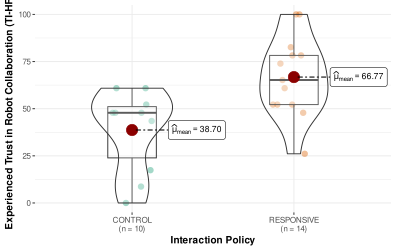
\includegraphics[keepaspectratio]{misty-paper_files/figure-pdf/fig-post-eligible2-1.pdf}}

}

\caption{\label{fig-post-eligible2}Distribution of Trust in Industrial
Human--Robot Collaboration scores by interaction policy. Points
represent individual observations; violins depict score distributions.
Red points indicate group means with 95\% confidence intervals.
Statistical comparisons are reported in the Results section.}

\end{figure}%

\paragraph*{Trust Perception
Scale--HRI}\label{trust-perception-scalehri}
\addcontentsline{toc}{paragraph}{Trust Perception Scale--HRI}

For the Trust Perception Scale--HRI, a comparable mixed-effects model
was fitted using the same fixed effects structure. In this model,
interaction with the responsive robot was associated with higher
post-interaction trust scores (β = 14.17, SE = 6.5, t = 2.00, p =
0.046). Effects of baseline negative attitudes toward robots and native
English fluency followed a similar directional pattern but did not
reliably differ from zero.

In contrast to the collaboration trust scale, inclusion of random
intercepts for individual trust items did not improve model fit for the
Trust Perception Scale--HRI and was therefore omitted. This divergence
likely reflects differences in scale format and response interface: the
Trust Perception scale was administered using a continuous slider input,
whereas the Trust in Industrial Human--Robot Collaboration scale
employed discrete Likert-style response options.

Informal observation during administration and post-hoc inspection of
item-level variance suggest that the slider-based interface,
administered via a touchpad, may have reduced response precision
relative to discrete response formats. While this likely attenuated
item-level variability, the Trust Perception Scale--HRI nevertheless
captured meaningful between-condition differences at the aggregate
level.

\begin{figure}

\centering{

\pandocbounded{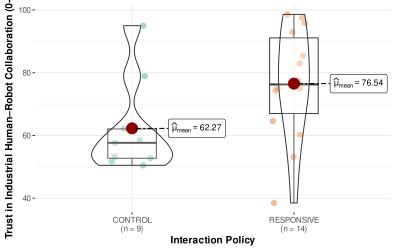
\includegraphics[keepaspectratio]{misty-paper_files/figure-pdf/fig-post-eligible-1.pdf}}

}

\caption{\label{fig-post-eligible}Distribution of Trust Perception in
HRI by interaction policy. Points represent individual observations;
violins depict score distributions. Red points indicate group means with
95\% confidence intervals. Statistical comparisons are reported in the
Results section.}

\end{figure}%

Together, these models indicate that robot responsiveness had a
consistent positive effect on post-interaction trust, with effect
magnitude and measurement sensitivity varying by trust dimension and
scale format.

\subsection{Bayesian analysis}\label{bayesian-analysis}

Trust outcomes were analysed using Bayesian linear mixed-effects models
to account for repeated measurement across trust items and sessions. Two
complementary trust measures were examined: task-oriented trust
(TPS-HRI), reflecting evaluative judgments of robot reliability and
competence, and experienced trust (TI-HRC), reflecting affective and
experiential aspects of collaboration. All models included random
intercepts for session and trust item. Convergence diagnostics indicated
satisfactory model performance across all analyses (all R\^{}≤1.01;
effective sample sizes \textgreater{} 1000).

Analyses are reported in three stages: (1) primary analyses conducted on
the eligible sample (n=24; sessions with viable spoken-language
interaction), (2) sensitivity analyses conducted on the full sample
(n=29; including sessions with severe communication breakdown), and (3)
mechanism analyses examining communication breakdown as a moderator of
interaction policy.

\subsubsection{Primary Analyses: Eligible
Sample}\label{primary-analyses-eligible-sample}

\paragraph*{Task-Oriented Trust
(TPS-HRI)}\label{task-oriented-trust-tps-hri}
\addcontentsline{toc}{paragraph}{Task-Oriented Trust (TPS-HRI)}

In the eligible sample (n=24), interaction policy showed a strong and
robust association with task-oriented trust. Participants who interacted
with the responsive robot reported higher TPS-HRI scores than those in
the control condition (posterior median β=12.73 credible interval
{[}2.93, 22.17{]}). The posterior probability that this effect was
positive exceeded 99\%, with high probability that the effect was of
moderate-to-large magnitude.

Baseline negative attitudes toward robots (NARS) were associated with
lower task-oriented trust, although uncertainty remained moderate and
the credible interval included zero. In contrast, native English fluency
showed a credible negative association with TPS-HRI scores, indicating
lower evaluative trust among non-native English speakers even in
sessions where dialogue remained viable.

The model explained a substantial proportion of variance in TPS-HRI
scores (conditional R2=0.64), with fixed effects accounting for
approximately 16\% of the variance. Random effects indicated meaningful
variability across sessions and trust items.

\paragraph*{Experienced Trust (TI-HRC)}\label{experienced-trust-ti-hrc}
\addcontentsline{toc}{paragraph}{Experienced Trust (TI-HRC)}

A similar but stronger pattern was observed for experienced trust.
Interaction with the responsive robot was associated with substantially
higher TI-HRC scores compared to the control condition (posterior median
β=14.86, 95\% credible interval {[}7.20, 22.09{]}), with near-unity
posterior probability of a positive effect and a high probability of a
large effect.

Baseline negative attitudes toward robots showed a clear and credible
negative association with experienced trust. Native English fluency was
also negatively associated with TI-HRC scores, although uncertainty was
greater and the credible interval narrowly overlapped zero.

Overall model fit was moderate (conditional R2=0.42), with fixed effects
explaining approximately 21\% of the variance. Compared to TPS-HRI,
item-level variance was smaller, suggesting greater coherence among
affective trust items under functional interaction conditions.

\subsection{Sensitivity Analyses: Full
Sample}\label{sensitivity-analyses-full-sample}

Sensitivity analyses were conducted including all sessions, regardless
of communication viability (n=29), to assess robustness of the primary
findings.

\paragraph*{Task-Oriented Trust
(TPS-HRI)}\label{task-oriented-trust-tps-hri-1}
\addcontentsline{toc}{paragraph}{Task-Oriented Trust (TPS-HRI)}

In the full sample, the posterior estimate for interaction policy
remained positive but was attenuated relative to the eligible sample
(posterior median β=7.04, 95\% credible interval {[}−1.83, 15.67{]}).
Although uncertainty increased and the credible interval included zero,
the posterior probability of a positive effect remained high
(\textgreater94\%).

Baseline negative attitudes toward robots continued to show a credible
negative association with TPS-HRI scores. The effect of native English
fluency was reduced and no longer credibly different from zero. Overall
model fit decreased relative to the eligible sample (conditional
R2=0.44), indicating increased unexplained variability when sessions
with severe communication breakdown were included.

\paragraph*{Experienced Trust
(TI-HRC)}\label{experienced-trust-ti-hrc-1}
\addcontentsline{toc}{paragraph}{Experienced Trust (TI-HRC)}

For experienced trust, attenuation effects were more pronounced. The
posterior estimate for interaction policy decreased substantially in the
full sample (posterior median β=7.17, 95\% credible interval {[}−1.97,
16.70{]}), with reduced probability of a large effect. Baseline negative
attitudes toward robots remained negatively associated with trust, while
the effect of native English fluency remained negative but uncertain.

Model fit remained moderate (conditional R2=0.60), but residual variance
increased, consistent with the inclusion of interactions in which
collaborative behaviour could not be sustained. These results indicate
that experienced trust is particularly sensitive to interaction
breakdown, and that trust ratings obtained under non-functional
interaction conditions do not reflect graded variation in collaborative
experience.

\subsection{Mechanism Analyses: Communication
Breakdown}\label{mechanism-analyses-communication-breakdown}

To examine whether communication quality altered how interaction policy
influenced trust, mechanism-focused analyses were conducted in the full
sample modelling proportional communication breakdown as a moderator of
interaction policy. These analyses were intended to isolate
interaction-level dynamics rather than participant characteristics.

\subsubsection*{Task-Oriented Trust
(TPS-HRI)}\label{task-oriented-trust-tps-hri-2}
\addcontentsline{toc}{subsubsection}{Task-Oriented Trust (TPS-HRI)}

For TPS-HRI, proportional communication breakdown showed weak and
unstable associations with trust. The posterior distribution of the
interaction between interaction policy and communication breakdown was
broad and centered near zero, indicating substantial uncertainty. This
suggests that evaluative trust judgments were relatively insensitive to
graded variation in communication quality once interaction viability was
established.

\subsubsection*{Experienced Trust
(TI-HRC)}\label{experienced-trust-ti-hrc-2}
\addcontentsline{toc}{subsubsection}{Experienced Trust (TI-HRC)}

In contrast, experienced trust showed a different pattern. Posterior
estimates indicated a consistent negative tendency for the interaction
between interaction policy and communication breakdown. While responsive
behaviour was associated with higher experienced trust under low levels
of breakdown, this advantage diminished as communication failures
accumulated. Although uncertainty remained high, the posterior
distribution indicated a meaningful probability that communication
breakdown attenuated the trust benefits of responsive behaviour.

Across analyses, responsive interaction policies were consistently
associated with higher trust, particularly when interaction functioned
as intended. Task-oriented trust appeared relatively robust to
communication degradation, whereas experienced trust was sensitive to
interaction-level failures and the robot's ability to sustain responsive
behaviour. Sensitivity and mechanism analyses indicate that
communication breakdown does not merely reduce trust uniformly, but
alters how interaction policy shapes the trust experience. These
findings support a distinction between trust as evaluative judgment and
trust as lived experience, and highlight the importance of modelling
interaction dynamics when evaluating trust in fully autonomous
human--robot collaboration.

Notably, under conditions of severe communication breakdown, the
RESPONSIVE robot continued to generate proactive assistance,
encouragement, and meta-communication aimed at repairing the
interaction. However, these efforts did not restore mutual understanding
and, in several cases, appeared to increase participant confusion and
cognitive load. In contrast, the CONTROL robot's reactive interaction
policy resulted in fewer unsolicited interventions, which---while less
supportive under normal conditions---reduced interaction complexity when
language-mediated collaboration was no longer viable.

As a result, trust ratings in non-viable sessions did not systematically
track the intended responsiveness manipulation. These findings suggest
that when spoken-language interaction collapses, higher-level constructs
such as trust and collaboration are no longer meaningfully instantiated.
Communication viability therefore represents a boundary condition for
evaluating affect-adaptive interaction policies in autonomous social
robots.

\subsection{Interaction dynamics and task
performance}\label{interaction-dynamics-and-task-performance}

\subsubsection{Task performance}\label{task-performance}

Objective task accuracy did not differ between conditions across any
task-level measures except suspect accuracy (robot dependendant task),
indicating that increased trust was only attributable to improved task
success when interaction was necessary to complete accurately.

ADD TABLE

Despite similar task accuracy, interactions in the responsive condition
were characterized by longer durations, slower response times, and a
higher number of AI-detected engaged responses. These findings suggest
that responsiveness altered the interaction dynamics and affective tone
rather than task outcomes.

\subsection{Individual differences and correlational
patterns}\label{individual-differences-and-correlational-patterns}

As expected, we found that higher Need for Cognition (NFC) scores were
negatively associated with Negative Attitudes Towards Robots (NARS),
indicating that individuals who enjoy effortful thinking tend to have
more positive attitudes towards robots. This relationship is consistent
with prior literature suggesting that cognitive engagement is associated
with openness to new technologies. In terms of NARS subscales, NFC was
negatively correlated with all three subscales, but significantly so
only in the domain of Situations of Interaction with Robots. This
suggests that individuals with higher NFC are less likely to hold
negative attitudes across various dimensions of robot interaction but
especially around direct interaction with robots.

--\textgreater{} how to talk about post-interaction correlations
w/pre-interaction measures Several behavioural and task-level measures
were correlated with post-interaction trust, consistent with the
interpretation that trust judgments were shaped by interaction quality;
these variables were not included as covariates in primary models to
avoid conditioning on potential mediators.

Baseline negative attitudes toward robots were negatively correlated
with post-interaction trust, with the strongest associations observed
for affective trust subscales. In contrast, objective task performance
was selectively associated with perceived reliability. Need for
cognition was negatively correlated with negative robot attitudes and
interaction-level negative affect, suggesting that individual
differences contributed to variability in trust responses.

\begin{figure}

\centering{

\pandocbounded{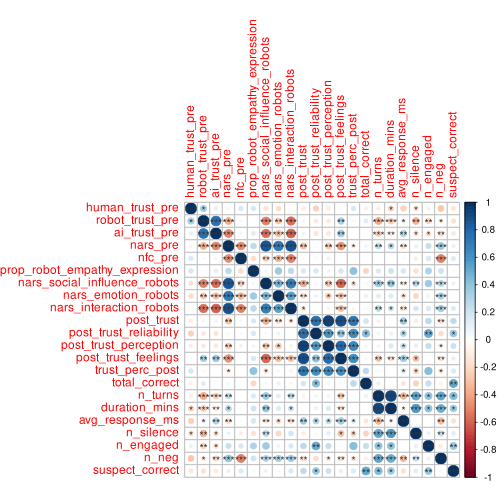
\includegraphics[keepaspectratio]{misty-paper_files/figure-pdf/fig-corr-1.pdf}}

}

\caption{\label{fig-corr}}

\end{figure}%

\begin{tcolorbox}[enhanced jigsaw, title=\textcolor{quarto-callout-important-color}{\faExclamation}\hspace{0.5em}{TO DO:}, titlerule=0mm, coltitle=black, bottomtitle=1mm, colframe=quarto-callout-important-color-frame, arc=.35mm, colbacktitle=quarto-callout-important-color!10!white, colback=white, breakable, opacitybacktitle=0.6, opacityback=0, leftrule=.75mm, toprule=.15mm, bottomrule=.15mm, toptitle=1mm, rightrule=.15mm, left=2mm]

CITATIONS

\begin{itemize}
\tightlist
\item
  add subscale column to long format data
\item
  run an analysis of performance by robot-dependent versus
  robot-independent tasks
\item
  write up a future directions section for the planned larger study
\item
  talk about unexpected language issues with people signing up with
  difficultly speaking and understanding english which cuased problems
  with asr and interaction
\item
  run analysis of dialogue dynamics included Bertopic or some other
  analysis of the actual content of the conversations/interactions
\end{itemize}

\end{tcolorbox}

\begin{tcolorbox}[enhanced jigsaw, title=\textcolor{quarto-callout-important-color}{\faExclamation}\hspace{0.5em}{TODO2}, titlerule=0mm, coltitle=black, bottomtitle=1mm, colframe=quarto-callout-important-color-frame, arc=.35mm, colbacktitle=quarto-callout-important-color!10!white, colback=white, breakable, opacitybacktitle=0.6, opacityback=0, leftrule=.75mm, toprule=.15mm, bottomrule=.15mm, toptitle=1mm, rightrule=.15mm, left=2mm]

Manually score each dialogue series.

For each interaction and stage:

\begin{itemize}
\tightlist
\item
  did the participant ask for help?
\item
  how many times?
\item
  did the robot give useful help?
\item
  did the robot give misleading or incorrect help?
\item
  did the robot stick to the policy?
\item
  how many times did the robot fail to understand the participant?
\end{itemize}

For each task:

\begin{itemize}
\tightlist
\item
  is there evidence that the robot helped complete the task?
\item
  is there evidence that the participant solved the problem without
  help?
\end{itemize}

\end{tcolorbox}

\section{Discussion}\label{discussion}

An additional objective of this pilot study was to inform the design of
an autonomous affect-adaptive interaction system under real-time
constraints. The initial system concept included multimodal affect
inference based on facial expressions, vocal prosody, and interaction
dynamics. However, early integration testing revealed substantial
challenges related to latency, model orchestration, and timing
sensitivity when deploying multiple perception models concurrently on an
edge-supported mobile robot platform. Given the small-scale nature of
the pilot and the central importance of maintaining stable, real-time
dialogue, the deployed system prioritized robustness of spoken-language
interaction and dialogue-based affect inference over broader multimodal
sensing. Affect adaptation in this study was therefore driven primarily
by speech-based affect signals and conversational context, allowing us
to evaluate responsiveness within a fully autonomous interaction while
preserving realistic system constraints.

The use of two trust instruments highlights an important distinction in
how trust is operationalized in HRI research. The Trust Perception
Scale--HRI emphasizes task-oriented and cognitive evaluations of system
performance, whereas the Trust in Industrial Human--Robot Collaboration
scale captures experiential and affective aspects of trust arising from
embodied interaction. While both measures converged on perceived
reliability, affective trust indicators were more strongly aligned with
behavioural engagement during interaction, suggesting that subjective
trust judgments alone may obscure how trust is enacted in practice.
Trust as judgement versus trust as experience.

Mention language confounders!! The present findings also highlight an
important boundary condition for trust measurement in spoken-language
HRI. When language-mediated interaction collapses entirely, higher-level
constructs such as trust and collaboration are no longer meaningfully
defined. Under such conditions, trust does not simply decrease; rather,
the interaction fails to instantiate the prerequisites necessary for
trust formation. This distinction is critical for both system evaluation
and experimental design, particularly as autonomous robots are deployed
in linguistically diverse, real-world environments.

Because the study relied fundamentally on spoken-language collaboration,
sessions exhibiting persistent communication failure were classified as
protocol non-adherence and excluded from task-level analyses (\emph{n} =
5). While the experimenter documented all cases where language might
pose an issue (as observed when meeting each participant), exclusion
decisions were based solely on actual communication viability and
interaction mechanics, not on task outcomes or trust measures.

The second task was intentionally designed to be sufficiently
challenging that completing it within the allotted time was difficult
without assistance. This ensured that interaction with the robot
represented a meaningful opportunity for collaboration rather than a
trivial or purely optional exchange. By contrasting a robot-dependent
task with an open-ended advisory task, the study examined trust
formation across interaction contexts that varied in both informational
asymmetry and reliance on the robot.

This pilot study examined trust outcomes following in-person interaction
with an autonomous social robot under two interaction policies: a
responsive, affect-adaptive condition and a neutral, non-responsive
control condition. By leveraging a fully autonomous dialogue system
integrated with speech recognition and affect detection, the study aimed
to evaluate how robot responsiveness influences trust formation in
realistic human--robot collaboration scenarios.

Descriptive comparisons of post-interaction measures indicated that
participants in the responsive condition reported consistently higher
trust across all trust measures, with differences ranging from
approximately 8 to 16 points on a 0--100 scale, although uncertainty
remained high given the small sample. Notably, the responsive condition
did not differ from control in objective task accuracy, suggesting that
increased trust was not driven by improved task success. Instead,
responsive interactions were characterized by longer durations, slower
response times, and a higher number of AI-detected engaged responses,
indicating a shift in interaction dynamics rather than performance.

Baseline negative attitudes toward robots were most strongly associated
with affective components of trust rather than perceptions of
reliability, suggesting that pre-existing attitudes primarily shape
emotional responses to interaction rather than judgments of system
competence. Conversely, objective task performance was selectively
associated with perceived reliability, indicating that participants
distinguished between affective and functional aspects of trust.

Future work with larger samples could formally test mediation pathways
linking robot responsiveness, interaction fluency, affective responses,
and trust judgments, as well as moderation by baseline attitudes toward
robots and need for cognition.

Participants in the responsive condition also exhibited higher levels of
AI-detected engagement during interaction, as indexed by a greater
number of responses classified as positive affect (t-test result). This
suggests that responsive behaviours altered the affective tone of the
interaction itself.

\subsection{Technical challenges}\label{technical-challenges}

Need to discuss that these items were on a 0-100 scale that required
sliding a bar, while the other trust scale was on a 1-5 Likert that
required simply clicking. The post test was administered on a laptop
with a trackpad which may have caused difficulties for some participants
who found it difficult to drag the slider with the trackpad. This could
have introduced additional noise into the measurement of this scale,
which may explain why the effects were somewhat weaker here.

\begin{itemize}
\tightlist
\item
  Need to talk about language issues with participants who had
  difficulty speaking and understanding English which caused problems
  with ASR and interaction.
\item
  Need to talk about issues where the AI was not able to flexibly handle
  when people asked a question about the suspect that was close to or
  another word for a ground-truth feature but not exactly the same word,
  causing confusion and miscommunication. E.g., ``Was the suspect
  wearing pink?'' The ground-truth feature was top: PINK, top-type:
  HOODIE; but the ASR and NLU did not extrapolate to understand that
  ``wearing pink'' referred to the same feature as ``top: PINK'',
  causing confusion and miscommunication. Maybe the prompt could have
  included some examples of different phrasing which could improve this?
  To solve this issue in future work, we can expand the NLU training
  data to include more paraphrases and synonyms for each feature.
\end{itemize}

There was also a case where someone asked `is the top shirt hoodie red?'
to which the AI answered YES. It may have been confused by the multiple
descriptors in the question. Future work could involve improving the NLU
to handle more complex queries with multiple attributes.

Discuss future work where we will look investigate the `embodied' effect
of having a physical robot versus a virtual agent on trust and
collaboration in HRI.

Also, prompt could include examples of what to do when dialogue appears
fragmented, to remind participants to wait until the blue light is on
before speaking and to switch up its phrasing if the robot seems to not
understand.

Also, the control condition seemed to be somewhat neutered in terms of
flexibility in responding in different ways. it would always respond
with the exact same phrase when confronted with a sentence fragment or a
question it could not directly answer.

Also issues with people not paying attention to the robot's visual cues
to know when to speak, leading to more fragmented dialogue. Future work
could involve improving participant instructions, improved latency and
`listening' \ldots{} and the robot's feedback mechanisms to better
manage turn-taking.

Need to remember to flag participants who did not complete/skipped
specific tasks. E.g. P56 skipped the wrapup entirely. Many skipped the
brief (by advancing on their own through the dashboard).

\section{Conclusion and Future Work}\label{conclusion-and-future-work}

\section{Appendix A}\label{sec-appendix-a}

\subsection{System Overview}\label{system-overview}

The experimental system comprised a fully autonomous, multi-stage
collaborative task in which participants interacted with the Misty II
social robot to solve a two-part investigative scenario. Interaction was
mediated through spoken dialogue and a companion web interface, allowing
the robot and participant to jointly reason about task information. The
system was designed as a mixed-initiative dialogue architecture with
optional affect-responsive behaviour, implemented without human
intervention during experimental sessions.

\subsection{Hardware Platform}\label{hardware-platform}

The robot platform used in this study was the Misty II social robot.
Misty II is a mobile social robot equipped with an expressive display,
articulated head and arms, and programmable RGB LEDs. These components
were used to produce synchronized verbal and nonverbal behaviour,
including eye expressions, head movements, arm gestures, and
colour-based state indicators. Audio input was captured via the robot's
RTSP video stream, which provided real-time access to the microphone
signal for downstream speech processing.

\subsection{Software Architecture}\label{software-architecture}

All system components were implemented in Python (version 3.10). The
software architecture integrated robot control, speech processing,
dialogue management, task logic, and data logging into a single
autonomous pipeline. Core dependencies included the Misty Robotics
Python SDK for robot control, the Deepgram SDK for speech recognition,
FFmpeg for audio stream processing, Flask and Flask-SocketIO for the
web-based task interface, and DuckDB for structured data logging.

\subsubsection{Dialogue Management and Large Language Model
Integration}\label{dialogue-management-and-large-language-model-integration}

Dialogue was managed using the LangChain framework, which provided
abstraction over message handling, memory persistence, and large
language model integration. The system used Google's Gemini API as the
underlying language model, configured to produce strictly JSON-formatted
outputs to ensure reliable downstream parsing and execution on the
robot.

The deployed model was \texttt{gemini-2.5-flash-lite}, selected for its
low-latency response characteristics. Generation temperature was set to
0.7 to balance coherence and variability. Conversation history was
maintained using a buffer-based memory mechanism, allowing the robot to
reference prior exchanges within a session while resetting memory
between participants. Conversation histories were stored as
session-specific JSON files to enable post-hoc analysis and recovery.

\subsubsection{Prompt Structure and Context
Injection}\label{prompt-structure-and-context-injection}

System prompts were constructed dynamically at each dialogue turn. Each
prompt consisted of a system message defining task rules, role
constraints, and output format requirements, followed by the accumulated
conversation history and the current participant utterance. In addition
to transcribed speech, structured contextual variables were injected
into the prompt as JSON fields, including the current task stage,
detected emotion labels, timer expiration flags, and task submission
status. This approach allowed the language model to access environmental
state without embedding control information directly into conversational
text.

\subsection{Speech Processing}\label{speech-processing}

Speech-to-text processing was handled by Deepgram's Nova-2 model using
real-time WebSocket streaming. The system employed adaptive endpointing
and voice activity detection to support conversational turn-taking.
Endpointing thresholds differed across task stages, with shorter
timeouts during dialogue-driven stages and longer timeouts during
log-reading phases.

Text-to-speech output was generated using Misty II's onboard TTS engine,
which produces a synthetic robotic voice. Although external TTS options
(including OpenAI and Deepgram Aura voices) were implemented and tested,
the onboard voice was selected to avoid introducing human-like vocal
qualities that could independently influence trust perceptions.

\subsection{Emotion Detection and Affective State
Mapping}\label{emotion-detection-and-affective-state-mapping}

Participant affect was inferred from transcribed utterances using a
DistilRoBERTa-based emotion classification model fine-tuned for
English-language emotion detection. The model produced categorical
predictions (e.g., joy, frustration, anxiety, neutral), which were
mapped to higher-level interaction states such as positive engagement,
irritation, or confusion. In the responsive condition, these inferred
states were used to guide dialogue strategy and nonverbal behaviour
selection.

\subsection{Multimodal Behaviour
Generation}\label{multimodal-behaviour-generation}

The robot's nonverbal behaviour was implemented through a library of
custom action scripts combining facial expressions, LED patterns, arm
movements, and head motions. At each dialogue turn, the language model
selected an expression label from a predefined set, which was then
translated into a coordinated multimodal action. In the responsive
condition, additional backchannel behaviours were triggered during
participant speech, including listening cues and emotion-matched
expressions.

LED colours were used to signal system state to participants. A blue LED
indicated active listening, while a purple LED indicated processing or
speaking.

\subsection{Collaborative Tasks}\label{collaborative-tasks}

The interaction consisted of two collaborative tasks. In the first task,
participants and the robot jointly solved a ``who-dunnit'' problem by
eliminating suspects from a grid based on yes/no questions. The robot
possessed ground-truth knowledge but was constrained to answering only
feature-based yes/no queries. In the second task, participants and the
robot attempted to locate a missing robot by interpreting cryptic system
and sensor logs. In this task, the robot did not know the solution and
instead provided guidance based on general technical knowledge and
logical reasoning.

Task information and participant responses were presented through a
web-based dashboard. The dashboard displayed suspect grids, system logs,
and response input fields, and communicated task progression events back
to the robot via REST API calls.

\subsection{Data Collection and
Logging}\label{data-collection-and-logging}

All interaction data were logged to a DuckDB relational database. Logged
data included session metadata, turn-level dialogue transcripts,
language model responses, nonverbal behaviour selections, response
latencies, task submissions, detected emotions, and system events such
as stage transitions and timer expirations. This structure enabled
detailed post-hoc analysis of interaction dynamics, communication
failures, and trust-related behaviours.

\subsection{Interaction Dynamics and Control
Modes}\label{interaction-dynamics-and-control-modes}

Two interaction policies were implemented and toggled programmatically
at runtime: a responsive mode and a control mode. In the responsive
mode, the robot proactively offered assistance, adjusted its dialogue
based on inferred affect, and produced supportive backchannel
behaviours. In the control mode, the robot provided information only
when explicitly prompted and did not adapt its behaviour based on
affective cues. The active mode was set prior to each session and
remained fixed throughout the interaction.

Silence handling was implemented using a fixed threshold, after which
the robot issued a check-in prompt. The phrasing of these prompts
differed across conditions to reflect proactive versus reactive
interaction strategies.

\subsection{Inter-process
Communication}\label{inter-process-communication}

System components communicated via a set of Flask-based REST endpoints.
These endpoints synchronized task stage state, detected participant
submissions, managed timer events, and allowed limited facilitator
override when necessary. All communication between the web interface and
the robot occurred locally to ensure low latency and experimental
reliability.

\section{Appendix B}\label{sec-appendix-b}

\subsection{\texorpdfstring{Trust Perception Scale--HRI (TPS-HRI;
adapted
\citep{schaefer2016})}{Trust Perception Scale--HRI (TPS-HRI; adapted {[}@schaefer2016{]})}}\label{trust-perception-scalehri-tps-hri-adapted-schaefer2016}

Participants rated the following items on a percentage scale (0--100\%),
indicating the proportion of time each statement applied to the robot
during the interaction.

\begin{itemize}
\tightlist
\item
  What percent of the time was the robot dependable?
\item
  What percent of the time was the robot reliable?
\item
  What percent of the time was the robot responsive?
\item
  What percent of the time was the robot trustworthy?
\item
  What percent of the time was the robot supportive?
\item
  What percent of the time did this robot act consistently?
\item
  What percent of the time did this robot provide feedback?
\item
  What percent of the time did this robot meet the needs of the mission
  task?
\item
  What percent of the time did this robot provide appropriate
  information?
\item
  What percent of the time did this robot communicate appropriately?
\item
  What percent of the time did this robot follow directions?
\item
  What percent of the time did this robot answer the questions asked?
\end{itemize}

\subsection{\texorpdfstring{Trust in Industrial Human--Robot
Collaboration (TI-HRC; adapted
\citep{charalambous2016})}{Trust in Industrial Human--Robot Collaboration (TI-HRC; adapted {[}@charalambous2016{]})}}\label{trust-in-industrial-humanrobot-collaboration-ti-hrc-adapted-charalambous2016}

Participants indicated their agreement with the following statements
using a 5-point Likert-type scale. Negatively worded items were
reverse-scored prior to analysis.

\textbf{\emph{Reliability}}

\begin{itemize}
\tightlist
\item
  I trusted that the robot would give me accurate answers.
\item
  The robot's responses seemed reliable.
\item
  I felt I could rely on the robot to do what it was supposed to do.
\end{itemize}

\textbf{\emph{Perceptual / Affective Trust}}

\begin{itemize}
\tightlist
\item
  The robot seemed to enjoy helping me.
\item
  The robot was responsive to my needs.
\item
  The robot seemed to care about helping me.
\end{itemize}

\textbf{\emph{Discomfort / Unease}}

\begin{itemize}
\tightlist
\item
  The way the robot moved made me uncomfortable. (R)
\item
  The way the robot spoke made me uncomfortable. (R)
\item
  Talking to the robot made me uneasy. (R)
\end{itemize}

\section{Appendix C}\label{sec-appendix-b}

\subsection{Dialogue Coding Scheme}\label{dialogue-coding-scheme}

\subsubsection{Task Outcome Layer
(Stage-Level)}\label{task-outcome-layer-stage-level}

\begin{longtable}[]{@{}
  >{\raggedright\arraybackslash}p{(\linewidth - 4\tabcolsep) * \real{0.3750}}
  >{\raggedright\arraybackslash}p{(\linewidth - 4\tabcolsep) * \real{0.2500}}
  >{\raggedright\arraybackslash}p{(\linewidth - 4\tabcolsep) * \real{0.3750}}@{}}
\toprule\noalign{}
\begin{minipage}[b]{\linewidth}\raggedright
Variable
\end{minipage} & \begin{minipage}[b]{\linewidth}\raggedright
Type
\end{minipage} & \begin{minipage}[b]{\linewidth}\raggedright
Description
\end{minipage} \\
\midrule\noalign{}
\endhead
\bottomrule\noalign{}
\endlastfoot
\texttt{task\_outcome} & categorical & Final task status
(\texttt{completed}, \texttt{timeout}, \texttt{skipped},
\texttt{partial}, \texttt{abandoned}). \\
\texttt{task\_completed} & binary & Task goal was fully completed. \\
\texttt{task\_timed\_out} & binary & Task ended due to expiration of the
time limit. \\
\texttt{task\_skipped} & binary & Participant explicitly skipped or
advanced past the stage. \\
\texttt{task\_partially\_completed} & binary & Task progress was made,
but the full solution was not reached. \\
\texttt{task\_abandoned} & binary & Participant disengaged or stopped
attempting the task before timeout. \\
\texttt{task\_completed\_without\_help} & binary & Task was completed
without any help requests to the robot. \\
\texttt{task\_required\_robot\_help} & binary & At least one robot help
interaction was required for task completion. \\
\end{longtable}

\subsection{Dialogue Interaction Layer
(Turn-Level)}\label{dialogue-interaction-layer-turn-level}

\subsubsection*{Human Turn Codes}\label{human-turn-codes}
\addcontentsline{toc}{subsubsection}{Human Turn Codes}

\begin{longtable}[]{@{}
  >{\raggedright\arraybackslash}p{(\linewidth - 4\tabcolsep) * \real{0.3750}}
  >{\raggedright\arraybackslash}p{(\linewidth - 4\tabcolsep) * \real{0.2500}}
  >{\raggedright\arraybackslash}p{(\linewidth - 4\tabcolsep) * \real{0.3750}}@{}}
\toprule\noalign{}
\begin{minipage}[b]{\linewidth}\raggedright
Variable
\end{minipage} & \begin{minipage}[b]{\linewidth}\raggedright
Type
\end{minipage} & \begin{minipage}[b]{\linewidth}\raggedright
Description
\end{minipage} \\
\midrule\noalign{}
\endhead
\bottomrule\noalign{}
\endlastfoot
\texttt{human\_help\_request} & binary & Participant explicitly or
implicitly asks the robot for help or guidance. \\
\texttt{human\_reasoning} & binary & Participant reasons out loud with
the robot toward problem-solving. \\
\texttt{human\_confusion} & binary & Participant expresses confusion or
uncertainty. \\
\texttt{human\_confirmation\_seeking} & binary & Participant seeks
confirmation of a tentative belief or solution. \\
\end{longtable}

\subsubsection*{Robot Turn Codes}\label{robot-turn-codes}
\addcontentsline{toc}{subsubsection}{Robot Turn Codes}

\begin{longtable}[]{@{}
  >{\raggedright\arraybackslash}p{(\linewidth - 4\tabcolsep) * \real{0.3889}}
  >{\raggedright\arraybackslash}p{(\linewidth - 4\tabcolsep) * \real{0.2500}}
  >{\raggedright\arraybackslash}p{(\linewidth - 4\tabcolsep) * \real{0.3611}}@{}}
\toprule\noalign{}
\begin{minipage}[b]{\linewidth}\raggedright
Variable
\end{minipage} & \begin{minipage}[b]{\linewidth}\raggedright
Type
\end{minipage} & \begin{minipage}[b]{\linewidth}\raggedright
Description
\end{minipage} \\
\midrule\noalign{}
\endhead
\bottomrule\noalign{}
\endlastfoot
\texttt{robot\_helpful\_guidance} & binary & Robot provides accurate,
task-relevant information or guidance. \\
\texttt{robot\_misleading\_guidance} & binary & Robot provides
misleading or incorrect guidance. \\
\texttt{robot\_factually\_incorrect} & binary & Robot states information
that is objectively incorrect (though it may not know it is
incorrect). \\
\texttt{robot\_policy\_violation} & binary & Robot violates stated
system or task constraints. \\
\texttt{robot\_on\_policy\_unhelpful} & binary & Robot adheres to policy
but provides vague or non-actionable assistance. \\
\texttt{robot\_stt\_failure} & binary & Robot response reflects a
speech-to-text or input understanding failure. \\
\texttt{robot\_clarification\_request} & binary & Robot asks the
participant for information or to repeat or clarify their input. \\
\end{longtable}

\subsection{Affective Interaction Layer
(Turn-Level)}\label{affective-interaction-layer-turn-level}

\subsubsection*{Robot Affective
behaviour}\label{robot-affective-behaviour}
\addcontentsline{toc}{subsubsection}{Robot Affective behaviour}

\begin{longtable}[]{@{}
  >{\raggedright\arraybackslash}p{(\linewidth - 4\tabcolsep) * \real{0.3889}}
  >{\raggedright\arraybackslash}p{(\linewidth - 4\tabcolsep) * \real{0.2500}}
  >{\raggedright\arraybackslash}p{(\linewidth - 4\tabcolsep) * \real{0.3611}}@{}}
\toprule\noalign{}
\begin{minipage}[b]{\linewidth}\raggedright
Variable
\end{minipage} & \begin{minipage}[b]{\linewidth}\raggedright
Type
\end{minipage} & \begin{minipage}[b]{\linewidth}\raggedright
Description
\end{minipage} \\
\midrule\noalign{}
\endhead
\bottomrule\noalign{}
\endlastfoot
\texttt{robot\_empathy\_expression} & binary & Robot expresses empathy,
encouragement, or reassurance. \\
\texttt{robot\_emotion\_acknowledgement} & binary & Robot explicitly
references an inferred participant emotional state. \\
\end{longtable}

\subsubsection*{Human Affective
Response}\label{human-affective-response}
\addcontentsline{toc}{subsubsection}{Human Affective Response}

\begin{longtable}[]{@{}
  >{\raggedright\arraybackslash}p{(\linewidth - 4\tabcolsep) * \real{0.4028}}
  >{\raggedright\arraybackslash}p{(\linewidth - 4\tabcolsep) * \real{0.2500}}
  >{\raggedright\arraybackslash}p{(\linewidth - 4\tabcolsep) * \real{0.3472}}@{}}
\toprule\noalign{}
\begin{minipage}[b]{\linewidth}\raggedright
Variable
\end{minipage} & \begin{minipage}[b]{\linewidth}\raggedright
Type
\end{minipage} & \begin{minipage}[b]{\linewidth}\raggedright
Description
\end{minipage} \\
\midrule\noalign{}
\endhead
\bottomrule\noalign{}
\endlastfoot
\texttt{human\_affective\_engagement} & binary & Participant responds in
a socially warm or engaged manner. \\
\texttt{human\_social\_reciprocity} & binary & Participant mirrors or
responds to the robot's affective expression. \\
\texttt{human\_anthropomorphic\_language} & binary & Participant treats
the robot as a social agent. \\
\texttt{human\_emotional\_disengagement} & binary & Participant responds
in a curt, dismissive, or withdrawn manner. \\
\end{longtable}

\subsection{Notes}\label{notes}

\begin{itemize}
\tightlist
\item
  Turn-level variables are coded per dialogue turn.
\item
  Task outcome variables are coded once per
  \texttt{session\_id\ ×\ stage}.
\item
  Raw dialogue text was retained during coding and removed prior to
  aggregation.
\item
  Multiple turn-level codes may co-occur unless otherwise specified.
\end{itemize}


\bibliography{bibliography.bib}



\end{document}
